\documentclass{scrartcl}
\usepackage[utf8]{inputenc}
\usepackage{blindtext}
\usepackage{biblatex}
\bibliography{bibliography} 
\usepackage{booktabs}
\usepackage{pgfplots}
\usepackage{subcaption}


\title{Towards Paralleled N-Body Interaction}
\subject{INF560 Report}
\author{Zhengqing Liu  ~~Jiongyan Zhang}
\date{March 2022}

\begin{document}

\maketitle

\noindent \textbf{Abstract} The N-body problem has been widely studied and applied in various fields. Since the traditional Brute Force algorithm is computationally expensive and over time-consuming, the Barnes Hut quad-tree algorithm is proposed to simulate the particle force, which greatly improves the efficiency of the algorithm. Nowadays, the advent of parallel computing has given new born to these legacy algorithms. With MPI, OpenMP, and CUDA, we enforce parallelization at various degrees to experiment with the performance improvement upon Brute Force and Barnes Hut algorithms. The performance evaluation by exploiting different parallel paradigms as per the input scope are given in details.


\section{Introduction}
\noindent
N-body simulation consists of the evolution of a dynamic system of N bodies considering their mass, positions and initial speed, which is extensively used in astrophysics for studying how galaxies composed of millions of bodies behave~\cite{wiki}. 
Computers have been used to simulate N-body problems since the 1960s. 
Its main principle is based on Newtonian mechanics, simulating the force between each particle to calculate the direction and position at the next movement~\cite{aarseth2003gravitational}. 
As the computing power increases, multiple algorithms (i.e., Barnes Hut, etc.) are used to replace this basic algorithm~\cite{trenti2008n}. 
However, the development of computing power did not stop there. 
The availability of multicore processors has opened a new pan for high performance computing.
Parallelization unleashes the multi-thread or multi-process capabilities of CPUs and GPUs, along with distributed storage or shared storage, to divide and conquer so that the algorithm can leverage the computing power to solve the problem.

\noindent In the rest of this paper, we target at optimizing two classic algorithms (Brute Force and Barnes Hut) with several parallel paradigms, and evaluate the performance of various modes.

\section{Brute Force}
\noindent
Brute force is a naive algorithm that consists, for each time step, of computing the gravitational force applied to each particle, and then computing its new position respectively. 
The force applied to particle $p_1$ is computed by summing the force that all the other particles apply to $p_1$, which takes the complexity of $O(n^2)$.
Hence, the loops of force computation and position movement are the two essential parts to unleash the capability of parallelism.

\begin{figure}[!h]
\centering
\subcaptionbox{Original}{
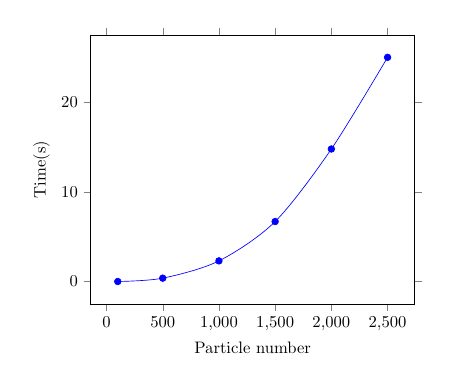
\begin{tikzpicture}[scale=0.6]
\begin{axis}[
    xlabel= Particle number,
    ylabel= Time(s),
    tick align=outside,
    legend style={at={(-0.2,0.6)},anchor=north}
    ]

\addplot[smooth,mark=*,blue] plot coordinates { 
    (100,0.0087)
    (500,0.3814)
    (1000,2.3094)
    (1500,6.7026)
    (2000,14.7978)
    (2500,25.0299)
};

\end{axis}
\end{tikzpicture}
}
\subcaptionbox{MPI}{
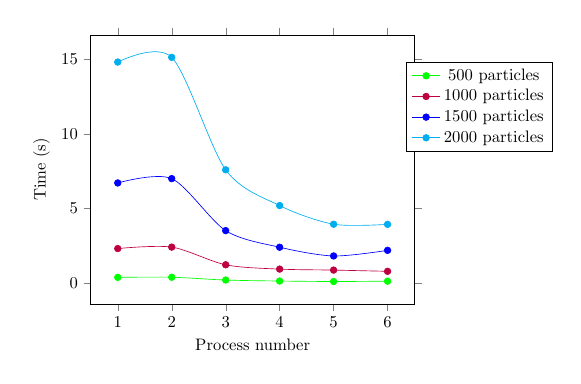
\begin{tikzpicture}[scale=0.6]

\begin{axis}[
    xlabel= Process number,
    ylabel= Time (s),
    tick align=outside,
    legend style={at={(1.2,0.9)},anchor=north}
    ]
\addplot[smooth,mark=*,green] plot coordinates { 
    (1,0.3814)
    (2,0.3894)
    (3,0.2012)
    (4,0.1356)
    (5,0.1034)
    (6,0.1249)
};
\addlegendentry{500 particles}

\addplot[smooth,mark=*,purple] plot coordinates { 
    (1,2.3094)
    (2,2.4071)
    (3,1.2224)
    (4,0.9334)
    (5,0.8675)
    (6,0.7857)
};

\addlegendentry{1000 particles}

\addplot[smooth,mark=*,blue] plot coordinates { 
    (1,6.7026)
    (2,6.992950)
    (3,3.511393)
    (4,2.398373)
    (5,1.814117)
    (6,2.189829)
};

\addlegendentry{1500 particles}

\addplot[smooth,mark=*,cyan] plot coordinates { 
    (1,14.7978)
    (2,15.114640)
    (3,7.583416)
    (4,5.188921)
    (5,3.939495)
    (6,3.930487)
};

\addlegendentry{2000 particles}

\end{axis}
\end{tikzpicture}
}
\caption{Orignal and MPI performance of Brute Force}
\label{fig:name}
\end{figure}

\subsection{MPI}
MPI (Message-Passing Interface)\footnote{https://www.mpi-forum.org/} is a message-passing library interface specification. 
It addresses primarily the message-passing parallel programming model, in which data is moved from the address space of one process to that of another process through cooperative operations on each process. 

\noindent To utilize the distributed-memory paradigm, we define a \textit{master} process and multiple \textit{slave} processes according to the given processes.
While slaves take force computation tasks equally, master finishes the modulo task and moves all the particles.
Collective communication, such as broadcast and gather,  facilitates the synchronization and collection. 
However, since the algorithm encompasses several arguments (i.e., force, velocity, position), synchronizing all of them would require broadcast with a couple of steps.
To this end, a new MPI datatype, \textit{particle\_mpi\_t}, is declared in our implementation, thus the whole particle structures can be transmitted at once. 
In case that the number of modulus task of master is not same as those of slave, gatherv is used to gather sets of particles in disparate lengths. 
In addition, the global variables, \textit{max\_acc} and \textit{max\_speed}, should also be updated among all the processes.

\subsection{MPI + OpenMP}
The OpenMP (Open Multi-Processing)\footnote{https://www.openmp.org/} supports multi-platform shared-memory parallel programming in C/C++ and Fortran.
To leverage both MPI and OpenMP for N-body problem, a fine-grain mode of hybrid programming is implemented - distribution of tasks over MPI ranks and process of each subpart with OpenMP.
Optimization of loop scheduling is a huge advantage of fine granurity.
In our scenarios, each slave rank computes the forces added up to a set of particles, which are specified by the master.
By creating omp parallel region for each slave, the for-loop of computing force can speed up. In this way, only few OpenMP constructs and clauses are involved and meanwhile relatively better performances are obtained. 

\noindent In addition, setting more than 4 processes, the performance is degraded along with the increment of the number of processes.
This phenomenon conforms to Amdahl's law.
Not only cannot the sequential portion be diminished, but launching and cooperating threads or processes takes costs. 


\begin{center}
\begin{table}
\footnotesize
\centering
\begin{subtable}[c]{0.7\textwidth}
\centering
\begin{tabular}{cccc}
\hline
Threads& 1000 particles& 2000 particles& 3000 particles\\
\hline
1& 2.587433& 16.243086& 43.273200\\
2& 2.336531& 14.792514& 39.182745\\
3& 2.255282& 15.018447& 42.185766\\
4& 2.411418& 15.249535& 42.789421\\
5& 2.452970& 14.749308& 43.151368\\
\hline
\end{tabular}
\subcaption{2 Processes}
\end{subtable}

\begin{subtable}[c]{0.7\textwidth}
\centering
\begin{tabular}{cccc}
\hline
Threads& 1000 particles& 2000 particles& 3000 particles\\
\hline
1& 1.327676& 8.315050& 23.706969\\
2& 1.894452& 11.965878& 33.056768\\
3& 1.790665& 10.809736& 28.787725\\
4& 1.654219& 9.455634& 24.729652\\
5& 4.189442& 9.502631& 24.380480\\
\hline
\end{tabular}
\subcaption{3 Processes}
\end{subtable}

\begin{subtable}[c]{0.7\textwidth}
\centering
\begin{tabular}{cccc}
\hline
Threads& 1000 particles& 2000 particles& 3000 particles\\
\hline
1& 0.899367& 5.583197& 15.528205\\
2& 1.586002& 9.062810& 24.073398\\
3& 1.414150& 6.780683& 22.774145\\
4& 4.471012& 9.574463& 23.262464\\
5& 5.686800& 12.974246& 26.736431\\
\hline
\end{tabular}
\subcaption{4 Processes}
\end{subtable}

\caption{MPI+OMP performance on Brute Force }
\end{table}
\end{center}
\subsection{MPI + OpenMP + CUDA}
CUDA is a parallel computing platform and application programming interface that allows software to use certain types of graphics processing unit for general purpose processing. 
With the acceleration of dedicated hardware, parallelism can step further.  

\noindent The unit task of computing all other forces upon one particle is transferred to CUDA. 
After allocating and copying memory to the device side, CUDA exploits its given blocks and threads to implement the force computation.
Due to the computed forces are added up in the various threads, the atomicity should be guaranteed to eschew the asynchronization. 
Typically, the built-in \textit{atomicAdd} is constrained to integer operations, thus rewriting the atomic adding for double type is necessary.
Inspired by Marco Bertini's solution~\cite{atomicAdd}, \textit{atomicAddDouble} is implemented to successfully execute double addition.

\noindent However, the performance is degraded with the involvement of CUDA.
And we observe that with the increment of processes, the speed further slows down.
Due to that OMP has trivial effects on the MPI version, we choose 2 omp threads and analyze the performance brought by CUDA. 
We choose \textit{thr\_per\_block} as 10, 50, 100 for 100, 500, 1000 particles scenarios respectively.

\begin{table}
\footnotesize
    \centering
    \begin{tabular}{cccc}
    \hline
    Processes& 100 particles& 500 particles& 1000 particles\\
    \hline
    2 (No CUDA)& 0.007055& 0.385060& 2.336531\\ 
    2& 0.631886& 13.081082& 78.902757\\
    3& 1.409775& 22.233090& 92.376449\\
    4& 1.477007& 22.345278& 109.797773\\
    \hline
    \end{tabular}
    \caption{Hybrid performance}
    \label{tab:my_label}
\end{table}

\section{Barnes Hut}
The Barnes Hut algorithm exploits the sparsity of particles to estimate the force on each particle. Instead of calculating the interaction force among each pair of particles, the algorithm treats the distant group of particles as one large particle and performs mechanical calculations with it~\cite{van2013barnes}. Via the approximate approach, one particle doesn't require to traverse all other particles.The core step in this algorithm is to establish a quad-tree, upon which one can gather space-neighbour particles~\cite{smith1994quad}.\\
The main idea of Barnes Hut parallelism is to make recursive structures loop. We mainly focus on the force computing part, as it is one of the most computing expensive steps and with the highest possibility to achieve parallelism~\cite{arnautovic2013parallelization}. The target is to separate the particles into several parts, which would be convenient for multiple threads or processes to handle independently. Meanwhile, we also try to use parallelism in the recursive function, aiming to finding a 
decent level to assign tasks to each thread.
The original non-parallel code possesses the performance as below.\\
\begin{figure}[!h]
\centering

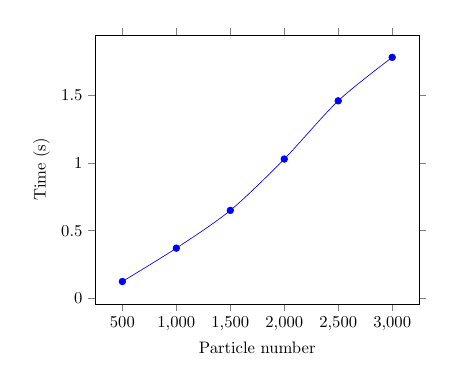
\begin{tikzpicture}[scale=0.6]

\begin{axis}[
    xlabel= Particle number,
    ylabel= Time (s),
    tick align=outside,
    legend style={at={(-0.2,0.6)},anchor=north}
    ]

\addplot[smooth,mark=*,blue] plot coordinates { 
    (500,0.1249)
    (1000,0.3709)
    (1500,0.6494)
    (2000,1.0282)
    (2500,1.4578)
    (3000,1.7784)
};

\end{axis}
\end{tikzpicture}
\caption{Original code performance of Barnes Hut}
\label{fig:name}
\end{figure}
\\It shows that with development of the particle number, the code operation time increases with an approximate-linear model. 

\subsection{MPI}
\noindent
Due to the distributed memory system and the complexity of a quad-tree structure, we cannot transfer the tree directly. Thus, we use more space for less time. The basic idea is to establish the tree in each process simultaneously. Finally, the tree in each process is the same as the initial parameters are shared. Each process could obtain a certain quantity of tasks in correspondence to the process number. Based on 1000 particles, we add the required process gradually and the result is showed in Figure 3.

\subsection{OpenMP}
\noindent
OpenMP provides a shared memory, thus the tree establishment in each thread is not required. We can just simply apply OpenMP for-loop with the dynamic mode. The parallelism mainly focuses on the force computing process. We try to increase the threads to examine the efficiency of OpenMP in this algorithm:
\begin{figure}[!h] 
\centering
\subcaptionbox{MPI}{
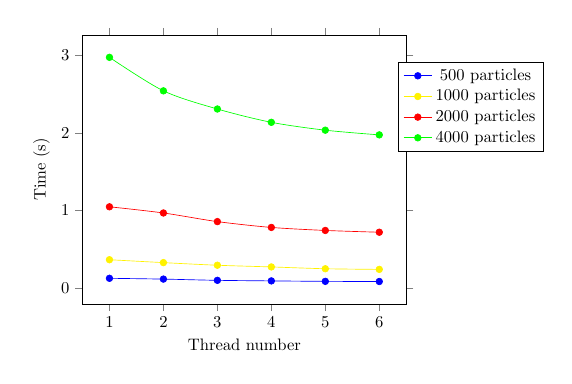
\begin{tikzpicture}[scale=0.6]

\begin{axis}[
    xlabel= Thread number,
    ylabel= Time (s),
    tick align=outside,
    legend style={at={(1.2,0.9)},anchor=north}
    ]
\addplot[smooth,mark=*,blue] plot coordinates { 
    (1,0.128103)
    (2,0.117752)
    (3,0.102021)
    (4,0.094662)
    (5,0.088839)
    (6,0.086950)
};

\addlegendentry{500 particles}

\addplot[smooth,mark=*,yellow] plot coordinates { 
    (1,0.367194)
    (2,0.329829)
    (3,0.296141)
    (4,0.274345)
    (5,0.250986)
    (6,0.242753)
};
\addlegendentry{1000 particles}

\addplot[smooth,mark=*,red] plot coordinates { 
    (1,1.048104)
    (2,0.968597)
    (3,0.857459)
    (4,0.782523)
    (5,0.743836)
    (6,0.720818)
};

\addlegendentry{2000 particles}

\addplot[smooth,mark=*,green] plot coordinates { 
    (1,2.970725)
    (2,2.539754)
    (3,2.306051)
    (4,2.134788)
    (5,2.033596)
    (6,1.973217)
};

\addlegendentry{4000 particles}
%\addlegendentry{case 1}

\end{axis}
\end{tikzpicture}
}
\subcaptionbox{OMP}{
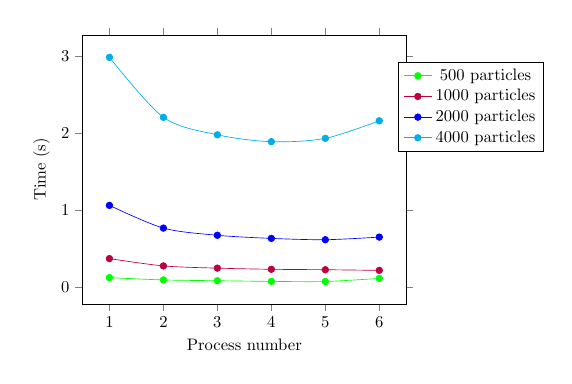
\begin{tikzpicture}[scale=0.6]

\begin{axis}[
    xlabel= Process number,
    ylabel= Time (s),
    tick align=outside,
    legend style={at={(1.2,0.9)},anchor=north}
    ]
\addplot[smooth,mark=*,green] plot coordinates { 
    (1,0.127127)
    (2,0.097437)
    (3,0.087053)
    (4,0.078695)
    (5,0.077142)
    (6,0.117528)
};
\addlegendentry{500 particles}

\addplot[smooth,mark=*,purple] plot coordinates { 
    (1,0.373572)
    (2,0.279013)
    (3,0.250259)
    (4,0.235290)
    (5,0.229734)
    (6,0.221141)
};

\addlegendentry{1000 particles}

\addplot[smooth,mark=*,blue] plot coordinates { 
    (1,1.062833)
    (2,0.768592)
    (3,0.675868)
    (4,0.635460)
    (5,0.618210)
    (6,0.652331)
};

\addlegendentry{2000 particles}

\addplot[smooth,mark=*,cyan] plot coordinates { 
    (1,2.980229)
    (2,2.203253)
    (3,1.977129)
    (4,1.887603)
    (5,1.931117)
    (6,2.158590)
};

\addlegendentry{4000 particles}

\end{axis}
\end{tikzpicture}
}
\caption{MPI and OMP performance in Barnes Hut}
\label{fig:name}
\end{figure}
\\The operating time decreases with the thread number increasing. However, it is clear that the speedup decreases, mainly because of the bus contention.

\subsection{Hybrid of MPI and OpenMP}
\noindent
The hybrid mode of MPI and OpenMP could provide a further choice for parallelism. The combination of two tools comes from the previous two sections. The top level design provides an MPI infrastructure, which follows the each-tree-each-process principle in 3.1 to create an environment for labour division. Inside each process, the for-loop could be parallelized by OpenMP.
\begin{figure}[!h] 
\centering
\subcaptionbox{500 particles}  
{  
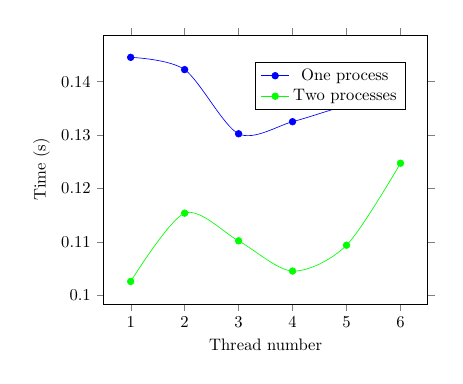
\begin{tikzpicture}[scale=0.6]

\begin{axis}[
    xlabel= Thread number, 
    ylabel= Time (s), 
    tick align=outside, 
    legend style={at={(0.7,0.9)},anchor=north} 
    ]

\addplot[smooth,mark=*,blue] plot coordinates { 
    (1,0.144559)
    (2,0.142259)
    (3,0.130231)
    (4,0.132497)
    (5,0.135561)
    (6,0.138098)
};


\addlegendentry{One process}

\addplot[smooth,mark=*,green] plot coordinates {
    (1,0.102542)
    (2,0.115353)
    (3,0.110164)
    (4,0.104497)
    (5,0.109342)
    (6,0.124713)
};
\addlegendentry{Two processes}

\end{axis}
\end{tikzpicture}
}
\subcaptionbox{1000 particles}  
{  
\centering
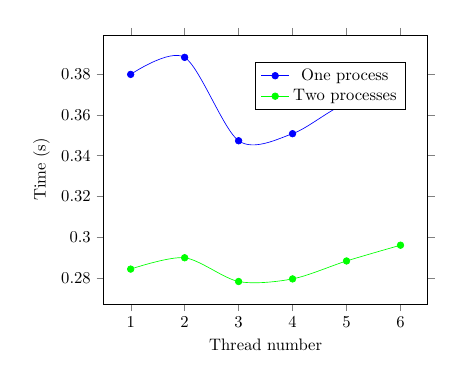
\begin{tikzpicture}[scale=0.6]

\begin{axis}[
    xlabel= Thread number, 
    ylabel= Time (s), 
    tick align=outside, 
    legend style={at={(0.7,0.9)},anchor=north} 
    ]

\addplot[smooth,mark=*,blue] plot coordinates { 
    (1,0.379917)
    (2,0.388298)
    (3,0.347317)
    (4,0.350786)
    (5,0.365727)
    (6,0.368501)
};


\addlegendentry{One process}

\addplot[smooth,mark=*,green] plot coordinates {
    (1,0.284265)
    (2,0.289831)
    (3,0.278172)
    (4,0.279449)
    (5,0.288258)
    (6,0.296005)
};
\addlegendentry{Two processes}


\end{axis}
\end{tikzpicture}
}
\subcaptionbox{2000 particles}  
{  
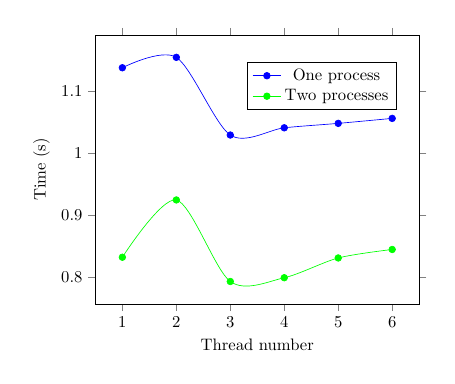
\begin{tikzpicture}[scale=0.6]

\begin{axis}[
    xlabel= Thread number, 
    ylabel= Time (s), 
    tick align=outside, 
    legend style={at={(0.7,0.9)},anchor=north} 
    ]

\addplot[smooth,mark=*,blue] plot coordinates { 
    (1,1.138275)
    (2,1.155056)
    (3,1.029712)
    (4,1.041404)
    (5,1.048535)
    (6,1.056574)
};


\addlegendentry{One process}

\addplot[smooth,mark=*,green] plot coordinates {
    (1,0.832576)
    (2,0.925001)
    (3,0.793431)
    (4,0.799537)
    (5,0.831406)
    (6,0.845097)
};
\addlegendentry{Two processes}

\end{axis}
\end{tikzpicture}
}
\subcaptionbox{4000 particles}  
{  
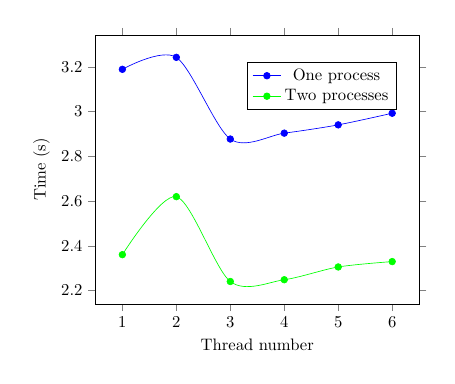
\begin{tikzpicture}[scale=0.6]

\begin{axis}[
    xlabel= Thread number, 
    ylabel= Time (s), 
    tick align=outside, 
    legend style={at={(0.7,0.9)},anchor=north} 
    ]

\addplot[smooth,mark=*,blue] plot coordinates { 
    (1,3.188606)
    (2,3.242111)
    (3,2.877078)
    (4,2.903363)
    (5,2.940451)
    (6,2.992418)
};


\addlegendentry{One process}

\addplot[smooth,mark=*,green] plot coordinates {
    (1,2.360512)
    (2,2.619732)
    (3,2.240612)
    (4,2.248531)
    (5,2.305573)
    (6,2.329586)
};
\addlegendentry{Two processes}

\end{axis}
\end{tikzpicture}
}
\caption{Hybrid performance of Barnes Hut}
\label{fig:name}
\end{figure}
\\We notice that there would be a time rising when applying the two threads. The possible reason is the additional thread cost.\\
\begin{figure}[!h]
\centering 

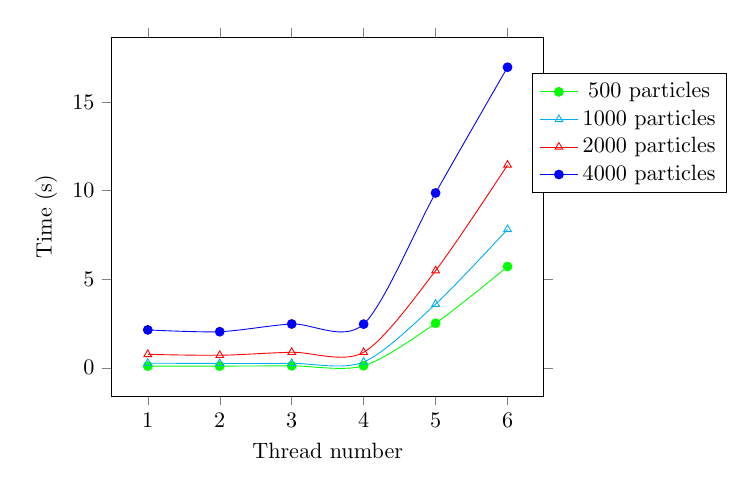
\begin{tikzpicture}[scale=0.8]

\begin{axis}[
    xlabel=Thread number, 
    ylabel=Time (s), 
    tick align=outside,
    legend style={at={(1.2,0.9)},anchor=north} 
    ]

\addplot[smooth,mark=*,green] plot coordinates { 
    (1,0.093081)
    (2,0.092248)
    (3,0.107316)
    (4,0.111796)
    (5,2.511965)
    (6,5.710171)
};

\addlegendentry{500 particles}

\addplot[smooth,mark=triangle,cyan] plot coordinates {
    (1,0.257285)
    (2,0.242022)
    (3,0.247034)
    (4,0.322218)
    (5,3.591909)
    (6,7.811057)
};
\addlegendentry{1000 particles}

\addplot[smooth,mark=triangle,red] plot coordinates {
    (1,0.755377)
    (2,0.704551)
    (3,0.873846)
    (4,0.871475)
    (5,5.479085)
    (6,11.445225)
};
\addlegendentry{2000 particles}

\addplot[smooth,mark=*,blue] plot coordinates { 
    (1,2.136210)
    (2,2.033896)
    (3,2.469436)
    (4,2.461708)
    (5,9.864239)
    (6,16.961032)
};

\addlegendentry{4000 particles}

\end{axis}
\end{tikzpicture}
\caption{Abnormal trend in three processes}
\label{fig:name}
\end{figure}
We can then find that the increment of processes and threads contributes to the program's acceleration. However, the abnormal trend appears, i.e., there would be a strange rise with three-process. The context switching of threads probably counts a main reason as the threads in use may exceed the limitation of the device.
\subsection{CUDA}
\noindent
Unlike MPI and OpenMP, the CUDA programming aims to utilizing numerous threads of GPU. The largest problem is how to transfer the tree structure from host to device. To simplify this problem, we try to establish the quad-tree on the device side directly. During the experiments, there are two problems: the stack space in GPU is relatively less, which could not support a normal establishment process; and, the computation of the normal-level amount of particles would be quite slower. Table 3 shows the efficiency of the algorithm based on 1000 and 2000 particles and that more threads lead to accelerate the program.
\begin{center}
\begin{table}
\footnotesize
\begin{center}
\begin{tabular}{ccc}
\hline
Thread number& 1000 particles& 2000 particles\\
\hline
20& 16.026382& 45.959570\\
1000& 14.313604& 40.887589\\
Demo (non-parallel)&0.398095&1.095418\\
\hline
\end{tabular}
\end{center}
\caption{CUDA performance on Barnes Hut}
\end{table}
\end{center}
As the Barnes Hut is not independently computation-intensive, while requiring more space than the normal algorithm like Brute Force, GPU can not have an obvious speed-up on the program; instead, the cost greatly worsens the algorithm outcome.

\subsection{Non-recursive algorithms}
\noindent
Non-recursive algorithms aims to solve the performance problem in CUDA. The main idea is to revise the recursive function to the non-recursive function. To fit the logic of Barnes Hut, Breadth-First Search is utilized to develop the non-recursive algorithm. A queue structure provides a container for the while-loop iteration search in the quad-tree.\\
The problem still exists. First, the algorithm could not facilitate the performance in CUDA (with similar time consumption); second, the heap overflow problem occurs.
\subsection{Other trials}
\noindent
\textbf{(a) Linear quad-tree}\\
The linear quad-tree is a strategy, which utilizes a 1D array where each index represents the Morton code of one 2D space cell. This structure is easy to be implemented and understood, which suits the particle separation and device or process transfer. However, one great drawback is that this method requires a large space to generate redundant space for the linear structure. \\ 
After the experiment, the compiler error indicates that the heap space is used out. There are two main problems: first, the requested length number has already exceeded the limitation of the INT type; second, we can notice that based on 1000 particles, the depth is around 15~20, which requires about $4^{14}\sim4^{19}$ cells for the array, which may be far more than the device burden limitation.\\
\textbf{(b) OMP task in recursion}\\
Though the recursion structure is not suitable for parallelism, OpenMP provides an \textit{omp task} function, which may take convenience for recursion parallelism. However, in our experiment, the time consumption would slightly rise if combined with \textit{omp task}. After granting each task operating condition (based on the node depth, forbidding deep omp tasks), we found in a more shadow level, less the time. We assume that the for-loop has already taken all the threads thus it might be a performance lose with the task.

\section{Conclusion}
In this work, we target at paralleling N-body simulation (Brute Force and Barnes Hut) with MPI, OpenMP and CUDA. 
In the Brute Force, MPI largely speeds up the computation, OpenMP provides slight enhancement in a fine-grain mode, while CUDA slows down the task at several magnitude of orders. 
In the Barnes Hut, the crucial point is to parallelize force computing as well. In face of a complex and huge tree structure, we can try to share the tree structure in the memory space or build the same tree structure, using space to acquire a more efficient parallel algorithm. Meanwhile, the control of thread overhead also greatly affects the performance of the program. Besides, the CUDA model is not suitable for such a non-computation-intensive task, which largely degrades performance.
In both models, we observe the performance impairment when processes and threads are over some certain bounds.
Launching paralleled regions, communication among processes, copying memory to dedicated hardware all contributes to such degradation.

\def \articleBIBLIOGRAPHY{bibliography.bib}
\printbibliography

\end{document}

